\documentclass{AeroStructure-ERJohnson}
\input crosslink.tex

%\usepackage{showframe}
\def\ShowFrameLinethickness{0.125pt}

\def\harp#1{\smash{\mathord{\buildrel{\lower3pt\hbox{$\scriptscriptstyle\rightharpoonup$}}\over{#1}}}}

\myexternaldocument{App_4P}
\myexternaldocument{Ch01_4P}
\myexternaldocument{Ch02_4P}
\myexternaldocument{Ch03_4P}
\myexternaldocument{Ch04_4P}
%\myexternaldocument{Ch05_4P}
\myexternaldocument{Ch06_4P}
\myexternaldocument{Ch07_4P}
\myexternaldocument{Ch08_4P}
\myexternaldocument{Ch09_4P}
\myexternaldocument{Ch10_4P}
\myexternaldocument{Ch11_4P}
\myexternaldocument{Ch12_4P}
\myexternaldocument{Ch13_4P}
\myexternaldocument{Ch14_4P}
\myexternaldocument{Ch15_4P}
\myexternaldocument{Ch16_4P}
\myexternaldocument{Ch17_4P}
\myexternaldocument{Ch18_4P}


\begin{document}

\mainmatter

%\hbox{~}\clearpage
\setcounter{page}{121}


\setcounter{chapter}{4}

\chapter[Work and energy methods]{Work and energy\break methods}\label{chap05}

In article \ref{sec5.1} and article \ref{sec5.2} Hooke's law is presented in terms of generalized forces and their corresponding generalized displacements acting on a body. Refer to eqs. (\ref{eq5.6}) and (\ref{eq5.10}). Corollaries to Hooke's law are the principle of superposition and the reciprocal theorem of Maxwell. Articles \ref{sec5.3} to \ref{sec5.6} develop expressions for the energy stored due to elastic deformation of a thin-walled bar. Castigliano's energy theorems are presented in articles \ref{sec5.7} and~\ref{sec5.8}.

\section{Hooke's law and its corollaries}\label{sec5.1}

Consider a body, or structure, supported so that rigid body motion is impossible. If it subject to a force, say by hanging a weight on it, then by Newton's law of action-reaction the body must resist the force by producing an equal and opposite force. The manner by which the body produces this reactive force is by deforming. That is, the body changes shape under the action of a mechanical force and it is the change in shape that enables it to supply the reactive force. If the force is removed and the body returns to its original shape, then the body is\break \textbf{elastic}.

\begin{wrapfigure}[10]{R}{113pt}
\vspace{-17pt}
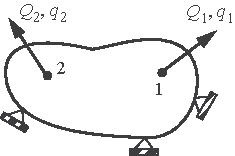
\includegraphics{Figure_5-1.pdf}
\caption{Static equilibrium of a body under external forces.\label{fig5.1}}
\end{wrapfigure}

 Consider the action of force $Q_{1}$ at point 1 on the body, and the action of force $Q_{2}$ at point 2 on the body shown in figure~\ref{fig5.1}. Let the forces be fixed in direction and in point of application. Let the displacements at points 1 and 2 be denoted by $q_{1}$ and $q_{2}$, respectively, being measured with respect to a rectangular Cartesian reference frame. Define the displacements $q_{1}$ and $q_{2}$ at the points of application to be in the direction of the forces $Q_{1}$ and $Q_{2}$, respectively. Displacements $q_{i}$ and forces $Q_{i}$, $i=1,2$, are said to \textbf{correspond}; \textit{they are defined at the same point and in the same direction}.

For a linear elastic body Hooke's law governs the response (Robert Hooke, 1635–1703). If only force $Q_1$ is applied, Hooke's law is
\begin{gather}\label{eq5.1}
\begin{array}{@{}ll@{}}
q_{1}=c_{11} Q_{1} & \text { for } Q_{2}=0 \\[4pt]
q_{2}=c_{21} Q_{1} & \text { for } Q_{2}=0
\end{array}.
\end{gather}
If force only force $Q_2$ is applied, Hooke's law is\vspace*{-4pt}
\begin{gather}\label{eq5.2}
\begin{array}{@{}ll@{}}
q_{1}=c_{12} Q_{2} & \text { for } Q_{1}=0 \\[4pt]
q_{2}=c_{22} Q_{2} & \text { for } Q_{1}=0
\end{array}.
\end{gather}
The coefficients $c_{11}$, $c_{12}$, $c_{21}$, and $c_{22}$ are called \textbf{flexibility influence coefficients}, and they depend on the points of application and the direction of the corresponding forces and displacements, and the size, shape, and the material of the body.

Note that\enlargethispage{0.6\baselineskip} the application of the force $Q_1$ results in a displacement at point 2, and force $Q_2$ results in a displacement at point 1. Under mechanical load Hooke recognized that the material from which the body is made deforms internally throughout its extent. We now know the scale of deformation is to the level of the distortion of interatomic bonds constituting the material. At the atomic scale the material is not continuous. However, for length scales greater than that of interatomic distances the atomic structure of the body is ignored and the body is idealized as a \textbf{continuum}. Points within the body are identified with the material particles, and continuity is defined in the mathematical sense. Neighboring points remain neighbors under any loading condition.

If both forces $Q_1$ and $Q_2$ act on the body, a questions that arises: Is Hooke's law given by eq.~(\ref{eq5.3}) below?\vspace*{-4pt}
\begin{gather}\label{eq5.3}
\begin{array}{@{}l@{}}
q_{1}=c_{11} Q_{1}+c_{12} Q_{2} \\[4pt]
q_{2}=c_{21} Q_{1}+c_{22} Q_{2}
\end{array}.
\end{gather}
From the hypothesis that the body returns to its original shape after the forces are removed it is proved that eq.~(\ref{eq5.3}) for two loads is the correct form of Hooke's law. The proof is given by Fung (1965, p.~3). Also, coefficients $c_{11}$ and $c_{21}$ are independent of force $Q_2$, and coefficients $c_{12}$ and $c_{22}$ are independent of force $Q_1$. This proof leads to the principle of superposition.

\begin{framed}
\noindent\textbf{Principle of superposition}\\
\hspace*{-10pt}\rule{37.45pc}{2pt}
\textbf{For a linear elastic body the effects caused by two or more loads are the sum of the loads applied separately.}\vspace*{-6pt}
\begin{itemize}
\item The deformations are small, and
\item the order of loading is unimportant.\vspace*{-5pt}
\end{itemize}
\end{framed}

\subsection{Work of the external loads}\label{sec5.1.1}


Multiplying the first of eq.~(\ref{eq5.3}) by $Q_{1}$, the second equation by $Q_{2}$, and adding, we obtain

\begin{wrapfigure}[5]{L}{156pt}
\vspace*{15pt}
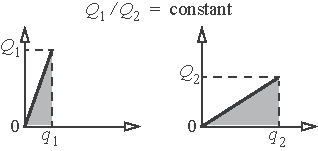
\includegraphics{Figure_5-2.pdf}
\caption{Load-displacement plots for proportional loading. \label{fig5.2}}
\vspace*{-25pt}
\end{wrapfigure}

\vspace*{-2.3pc}

\begin{align}\label{eq5.4}
Q_{1} q_{1}+Q_{2} q_{2}=c_{11} Q_{1}^{2}+c_{12} Q_{1} Q_{2}+c_{21} Q_{2} Q_{1}+c_{22} Q_{2}^{2} .
\end{align}

\vspace*{-1pc}

\noindent The quantity above is independent of the order in which the loads are applied. Hence, it has a definite meaning for each order of the application of loads $Q_1$ and $Q_2$.

Consider the special case of proportional loading, where the ratio $Q_2/Q_1$ is kept constant and the loading increases very slowly from zero to the final value (i.e., \textbf{quasi-static loading)}. In this case, the corresponding displacements also increase proportionally and slowly. Force-displacement plots at points 1 and 2 are shown in figure~\ref{fig5.2}\vadjust{\vspace*{10pt}\clearpage} for this special case of proportional loading. It should be clear that the work done by the force $Q_{1}$ is exactly $ \frac{1}{2} Q_{1} q_{1} $, and that of $Q_{2}$ is $\frac{1}{2} Q_{2} q_{2}$.



Hence, we conclude from eq.~(\ref{eq5.4}) that the \textbf{total work done, W, by the set of forces is independent of the order in which the forces are applied.}
\begin{align}\label{eq5.5}
W=\frac{1}{2}\left(Q_{1} q_{1}+Q_{2} q_{2}\right) .
\end{align}

\subsection{Maxwell's reciprocal theorem}\label{sec5.1.2}

Now consider the two different sequences in the application of forces $Q_1$ and $Q_2$. First, apply $Q_{1}$ slowly with $Q_{2}=0 $. At the final value of $Q_{1} $, the displacement of point 1 is $ c_{11} Q_{1} $ and the displacement of point 2 is $ c_{21} Q_{1} $. The work done is $ \frac{1}{2} c_{11} Q_{1}^{2} $. With $Q_{1}$ held fixed, apply $Q_{2}$ slowly until $Q_{2}$ attains its final value. The additional displacement at point 1 is $ c_{12} Q_{2} $ and the additional displacement at point 2 is $ c_{22} Q_{2} $. The additional work done is $ Q_{1} c_{12} Q_{2}+\frac{1}{2} c_{22} Q_{2}^{2} $. When the forces are applied in the order $ Q_{1}, Q_{2} $, the total work done, as shown in figure~\ref{fig5.3},~is
\begin{align*}
W=\underbrace{\frac{1}{2} c_{11} Q_{1}^{2}+c_{12} Q_{1} Q_{2}}_{\text {pt. } 1}+\underbrace{\frac{1}{2} c_{22} Q_{2}^{2}}_{\text {pt. 2 }}.
\end{align*}

\processfigure{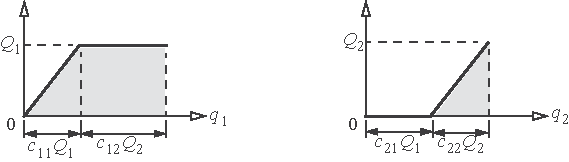
\includegraphics{Figure_5-3.pdf}}{\caption{Load-displacement plots for the loading sequence $Q_{\textbf{1}}$, $Q_{\textbf{2}}$.}\label{fig5.3}}

Second, apply $Q_{2}$ slowly with $ Q_{1}=0 $. At the final value of $Q_{2}$, the displacement of point 1 is $ c_{12} Q_{2} $ and the displacement of point 2 is $ c_{22} Q_{2} $. The work done is $ \frac{1}{2} c_{22} Q_{2}^{2} $. With $Q_{2}$ held fixed, apply $Q_{1}$ slowly until $Q_{1}$ attains its final value. The additional displacement at point 1 is $ c_{11} Q_{1} $ and the additional displacement at point 2 is $ c_{21} Q_{1} $. The additional work done is $ Q_{2} c_{21} Q_{1}+\frac{1}{2} c_{11} Q_{1}^{2} $. When the forces are applied in the order $ Q_{2}, Q_{1} $ the total work done, as shown in figure~\ref{fig5.4}, is
\begin{align*}
W^{\prime}=\underbrace{\frac{1}{2} c_{11} Q_{1}^{2}}_{{\rm pt.\ } 1}+\underbrace{\frac{1}{2} c_{22} Q_{2}^{2}+c_{21} Q_{1} Q_{2}}_{\rm {pt.\ } 2}.
\end{align*}

\processfigure{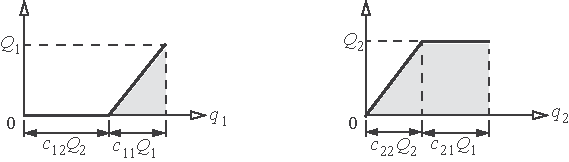
\includegraphics{Figure_5-4.pdf}}{\caption{Load-displacement plots\break for the loading sequence $Q_{\bf 2}$, $Q_{\bf 1}$.}\label{fig5.4}}

\pagebreak

\noindent However, $W=W^{\prime}$ for arbitrary order of application of $Q_{1},Q_{2}$. Hence, \fbox{$c_{12}=c_{21}$}.

For a set of applied forces $Q_{1}, Q_{2}, \ldots, Q_{n}$ and their corresponding displacements $ q_{1}, q_{2}, \ldots, q_{n} $, eq.~(\ref{eq5.3}) generalizes\vspace*{-6pt} to
\begin{align}\label{eq5.6}
q_{i}=\sum_{j=1}^{n} c_{i j} Q_{j} \quad i=1,2, \ldots, n.
\end{align}

\begin{framed}
\noindent\textbf{Maxwell's reciprocal theorem}\\
\hspace*{-10pt}\rule{37.45pc}{2pt}
\textbf{The influence coefficients for corresponding forces and displacements are symmetric.}\vspace*{-6pt}
\begin{itemize}
\item $c_{i j}=c_{j i}$\vspace*{-5pt}
\end{itemize}
\noindent\textbf{In other words, the displacement at point \textit{i} due to a unit load at another point \textit{j} is equal to the displacement at \textit{j} due to a unit load at \textit{i}, provided that the displacements and forces ``correspond,'' (i.e., that they are measured in the same direction at each point.)}
\end{framed}\vspace*{-6pt}

Since the flexibility influence coefficients $c_{12} = c_{21}$, the work done on the body can be written as
\begin{align}\label{eq5.7}
W=\frac{1}{2}\big(c_{11} Q_{1}^{2}+2 c_{12} Q_{1} Q_{2}+c_{22} Q_{2}^{2}\,\big).
\end{align}
Take the partial derivatives of the work function in eq.~(\ref{eq5.7}) with respect to forces $Q_1$ and $Q_2$, and recognize the material law in eq.~(\ref{eq5.3}), to find that
\begin{align}\label{eq5.8}
q_{1}=\frac{\partial W}{\partial Q_{1}} \quad q_{2}=\frac{\partial W}{\partial Q_{2}}.
\end{align}
That is, the partial derivative of the work function with respect to a force equals the corresponding displacement.

\section{Extensions of Hooke's law to include a couple and rotation}\label{sec5.2}

Hooke's law, eq.~(\ref{eq5.3}), can be extended to include the moment of a couple acting on the body and the rotation of the arm connecting the couple.

\begin{wrapfigure}[10]{R}{120pt}
\vspace{-19pt}
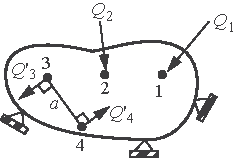
\includegraphics{Figure_5-5.pdf}
\caption{Static equilibrium of a body under external forces including a couple. \label{fig5.5}}
\end{wrapfigure}

As shown in figure~\ref{fig5.5}, the forces $ Q_{3}^{\prime} $ and $ Q_{4}^{\prime} $ form a couple with an arm of length $ a $ if $ Q_{3}^{\prime}=P $ and $ Q_{4}^{\prime}=P $. That is, forces $ Q_{3}^{\prime} $ and $ Q_{4}^{\prime} $ are functions of the force $ P $. Take the partial derivative of the work done by the forces with respect to force \textit{P} and use the chain rule to get
\begin{align*}
\frac{\partial W}{\partial P}=\frac{\partial W}{\partial Q_{3}^{\prime}} \frac{\partial Q_{3}^{\prime}}{\partial P}+\frac{\partial W}{\partial Q_{4}^{\prime}} \frac{\partial Q_{4}^{\prime}}{\partial P}.
\end{align*}
Let $ q_{3}^{\prime} $ denote the displacement corresponding to force $ Q_{3}^{\prime} $, and let $ q_{4}^{\prime} $ denote the displacement corresponding to force $ Q_{4}^{\prime} $. Then, with reference to eq.~(\ref{eq5.8}) $ q_{3}^{\prime}=\frac{\partial W}{\partial Q_{3}^{\prime}} $, $ q_{4}^{\prime}=\frac{\partial W}{\partial Q_{4}^{\prime}} $, and note that $ \frac{\partial Q_{3}^{\prime}}{\partial P}=\frac{\partial Q_{4}^{\prime}}{\partial P}=1 $. So
\begin{align*}
\frac{\partial W}{\partial P}=q_{3}^{\prime}+q_{4}^{\prime}.
\end{align*}

\begin{wrapfigure}[8]{R}{152pt}
%\vspace{-19pt}
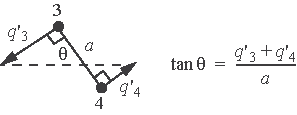
\includegraphics{Figure_5-6.pdf}
\caption{Rotation of the arm of the couple. \label{fig5.6}}
\end{wrapfigure}

\noindent For small displacements, $ q_{3}^{\prime}+q_{4}^{\prime}=a q $, where $q$ is the small rotation of the moment arm in radians, as is shown in figure~\ref{fig5.6}. Thus, $ \frac{\partial W}{\partial p}=a q $. Divide this last equation by the length of the moment arm to get\break $ \frac{1}{a} \frac{\partial W}{\partial P}=q $. Lastly, the moment of a couple is $ Q=a P $, so we get
\begin{align}\label{eq5.9}
\frac{\partial W}{\partial Q}=q .
\end{align}
Thus, in Hooke's law if $ q_{i}$ is a rotation, then corresponding ``force'' $Q_{i}$ is a moment.

We can consider a \textit{concentrated couple} as the limiting case of two equal and opposite forces acting in a plane at the surface of the body that approach each other, but maintain a constant moment; i.e.,
\begin{align*}
\underset{a \rightarrow 0}{\operatorname{Limit}}(a P)=Q
\end{align*}
In this limiting process $P \rightarrow \infty$. Then, the angle of rotation $q$ is interpreted as the rotation of an infinitesimal line element in the plane of the couple.

\subsection{Generalized forces and displacements}\label{sec5.2.1}

Define $Q_{i}$ as the magnitude of the generalized force acting at point $i$ on the body, and let $ q_{i} $ denote the corresponding generalized displacement at point $i$, where $ \dot{i}=1,2, \ldots, n $. The product of $ Q_{i} q_{i} $ has dimensional units of work, or \textit{F-L}. If $Q_{i}$ is a force, then $q_{i}$ is the corresponding displacement. If $Q_{i}$ is the moment of a concentrated couple with dimensional unit \textit{F-L}, then $q_{i}$ is the corresponding rotation in radians of the infinitesimal line element in the plane of the couple at the point of its application. By defining generalized forces and moments, we can extend Hooke's law in eq.~(\ref{eq5.6}) to include moments and rotations as well as forces and displacements. In eq.~(\ref{eq5.6}), the flexibility influence coefficients can have different dimensional units. For example, if $q_{1}$ is a displacement of point \textit{1} on the body and $Q_{2}$ is a moment of a couple acting point \textit{2}, then the dimensional unit of flexibility influence coefficient $ C_{12} $ is $ F^{-1} $. Since the generalized displacement $q_{2}$ corresponding to $Q_{2}$ is a rotation in radians and the generalized force $Q_{1}$ acting at point \textit{1} is a force corresponding to $q_{1}$, then the dimensional unit of flexibility influence coefficient $ c_{21} $ is also $ F^{-1} $. Also, the dimensional unit of $ c_{11}$ is $L F^{-1}$, and $c_{22}$ is $F^{-1} L^{-1}$.

\subsection{Stiffness influence coefficients}\label{sec5.2.2}

Assume that the displacement-force system given by eq.~(\ref{eq5.6}) can be inverted so that the forces may be expressed in terms of the displacements as
\begin{align}\label{eq5.10}
 Q_{i}=\sum_{j=1}^{n} k_{i j} q_{j} \quad i=1,2, \ldots, n ,
\end{align}
where constants $ k_{i j} $ are called \textbf{stiffness influence coefficients}. In matrix notation, we write the displacement-force form of Hooke's law, eq.~(\ref{eq5.6}), as
\begin{align}\label{eq5.11}
 \underbrace{\{q\}}_{n\, \times\, 1}=\underbrace{[c]}_{n\, \times\, n} \underbrace{\{Q\}}_{n\, \times\, 1} ,
\end{align}
and the force-displacement form, eq.~(\ref{eq5.10}), as
\begin{align}\label{eq5.12}
\underbrace{\{Q\}}_{n\, \times\, 1}=\underbrace{[k]}_{n \,\times \,n} \cdot \underbrace{\{q\}}_{n \,\times \,1} .
\end{align}
Matrix [$c$] is called the \textit{flexibility matrix} and [$k$] is called the \textit{stiffness matrix}. Both matrices are square of order $ n \times n $. In matrix algebra the stiffness matrix is the inverse of the flexibility matrix, or
\begin{align}\label{eq5.13}
[k]=[c]^{-1} .
\end{align}
The inverse matrix has the property that
\begin{align}\label{eq5.14}
[c]^{-1}[c]=[c][c]^{-1}=[I] ,
\end{align}
where [\textit{I}] is the $ n \times n $ identity matrix (i.e., the identity matrix is a square matrix with all diagonal elements equal to unity and all off-diagonal elements equal to zero).

Maxwell's theorem in article 5.1.2 states that the flexibility matrix is symmetric. In matrix algebra symmetry is written as
\begin{align}\label{eq5.15}
 [c]^{T}=[c] ,
\end{align}
where the superscript \textit{T} means matrix transpose (i.e., the matrix obtained by interchanging its rows with its columns). Since the flexibility matrix is symmetric, the stiffness matrix is also symmetric. That is,
\begin{align}\label{eq5.16}
 [k]^{T}=[k].
\end{align}

\begin{proof*}
By definition
\begin{align}\label{eq5.17}
 [c]^{-1}[c]=[I] .
\end{align}
Take the transpose of eq.~(\ref{eq5.17}) to get
\begin{align}\label{eq5.18}
 ([c]^{-1}[c])^{T}=[I]^{T} .
\end{align}
Use the fact that the transpose of the product of two matrices is equal to the product of the transpose of the second matrix times the transpose of the first matrix, and that the transpose of the identity matrix is equal to itself. Hence, eq.~(\ref{eq5.18}) is equal to
\begin{align}\label{eq5.19}
 [c]^{T}([c]^{-1})^{T}=[I] .
\end{align}
By symmetry of the flexibility matrix eq.~(\ref{eq5.19}) is equal to
\begin{align}\label{eq5.20}
 [c]([c]^{-1})^{T}=[I] .
\end{align}
Pre-multiply eq.~(\ref{eq5.20}) by the inverse of the flexibility matrix to get
\begin{align}\label{eq5.21}
 [c]^{-1}[c]([c]^{-1})^{T}=[c]^{-1}[I]=[c]^{-1} .
\end{align}
Employ the relation in eq.~(\ref{eq5.14}) and write eq.~(\ref{eq5.21}) as
\begin{align}\label{eq5.22}
([c]^{-1})^{T}=[c]^{-1}.
\end{align}
Again, by definition $[c]^{-1} \equiv[k]$. Thus,
\begin{align}\label{eq5.23}
 [k]^{T}=[k] .
\end{align}
\end{proof*}\hfill$\blacksquare$

Similarly in the generalized force and generalized displacement form of eq.~(\ref{eq5.12}), the stiffness influence coefficients, $k_{i j}$, also can have different dimensional units.
\vspace*{10pt}
\clearpage

\section{Strain energy density functions}\label{sec5.3}

External loads imposed on a body cause it to deform. The energy stored in an elastic body due to deformation is called the strain energy, and the strain energy per unit volume is called the strain energy density. For the thin wall bar theory discussed in article \ref{sec3.4} on page \pageref{sec3.4}, deformation is quantified by values of the axial normal strain $\varepsilon_{z z}$, and shear strains $\gamma_{z s}$ and $\gamma_{z \zeta}$. The three remaining strains $\varepsilon_{s s}=\varepsilon_{\zeta \zeta}=\gamma_{s \zeta}=0$. In this article expressions for the strain energy density functions in terms of the non-zero strains are developed.

\subsection{Strain energy density in uniaxial normal strain}\label{sec5.3.1}

Begin with the axial equation of motion for an element of the bar of length $\Delta z$ as shown in figure~\ref{fig5.7}. The equation of motion is

\processfigure{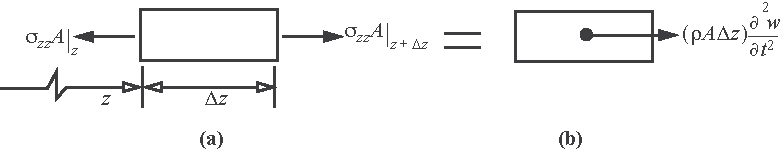
\includegraphics{Figure_5-7.pdf}}{\caption{Axial bar element. (a) free body diagram. (b) time rate of change of linear momentum.\vspace*{-1pc}}\label{fig5.7}}

\begin{align}\label{eq5.24}
\left.\sigma_{z z} A\right|_{z+\Delta z}-\left.\sigma_{z z} A\right|_{z}=(\rho A \Delta z) \frac{\partial^{2} w}{\partial t^{2}},
\end{align}
in which \textit{A} denotes the cross-sectional area, $\rho$ the mass density, and $\frac{\partial w}{\partial t}$ the axial velocity. Division of eq.~(\ref{eq5.24}) by $A\Delta z$ followed by letting $\Delta z \rightarrow 0$ yields the differential equation at coordinate $z$ and time $t$ as
\begin{align}\label{eq5.25}
\frac{\partial \sigma_{z z}}{\partial z}=\rho \frac{\partial^{2} w}{\partial t^{2}}.
\end{align}

\vspace*{-0.6pc}

Consider the first law of thermodynamics for a closed system of continuous matter not interchanging matter with its surroundings. Then the first law is (Malvern, 1969, p. 229)
\begin{align}\label{eq5.26}
P_{\text {input }}+Q_{\text {input }}=\frac{\partial E}{\partial t},
\end{align}
where $P_{\rm input}$ is the power input of the external loads, $Q_{\rm input}$ is the rate of heat input, and $E$ is the total energy of the system. Assume the process is \textbf{adiabatic} so $Q_{\rm input} = 0$. The energy is the sum of the kinetic energy and internal energy. For the closed system consisting of the axial bar element shown in figure~\ref{fig5.7}, $P_{\rm input}$ is the time rate of work of the normal stresses acting on the element. Expressions for $P_{\rm input}$ and the time rate of change of energy are
\begin{align}\label{eq5.27}
P_{\text {input }}=\left.\sigma_{z z} A \frac{\partial w}{\partial t}\right|_{z\,+\,\Delta z}-\left.\sigma_{z z} A \frac{\partial w}{\partial t}\right|_{z} \quad \frac{\partial E}{\partial t}=\frac{\partial}{\partial t}\left[\frac{1}{2}(\rho A \Delta z)\left(\frac{\partial w}{\partial t}\right)^{2}\right]+A \Delta z \frac{\partial U_{0}}{\partial t},
\end{align}
where $U_0$ is the internal energy per unit volume, or internal energy density. Substitute eq.~(\ref{eq5.27}) into the first law (\ref{eq5.26}) with $Q_{\rm input} = 0$, followed by division by $A\Delta z$. In the result from these previous manipulations let $\Delta z \rightarrow 0$ to get the differential equation of the first law at coordinate $z$ and time $t$ as\pagebreak
\begin{align}\label{eq5.28}
\frac{\partial}{\partial z}\left(\sigma_{z z} \frac{\partial w}{\partial t}\right)=\rho \frac{\partial w}{\partial t} \frac{\partial^{2} w}{\partial t^{2}}+\frac{\partial U_{0}}{\partial t}.
\end{align}
Expand the derivative on the left-hand side of eq.~(\ref{eq5.28}) to get
\begin{align}\label{eq5.29}
\frac{\partial \sigma_{z z}}{\partial z} \frac{\partial w}{\partial t}+\sigma_{z z} \frac{\partial}{\partial z}\left(\frac{\partial w}{\partial t}\right)=\rho \frac{\partial w}{\partial t} \frac{\partial^{2} w}{\partial t^{2}}+\frac{\partial U_{0}}{\partial t}.
\end{align}
Substitute the equation of motion (\ref{eq5.25}) for $\partial \sigma_{z z} / \partial z$ in the first term on the left-hand side of eq.~(\ref{eq5.29}). We assume it is permissible to interchange the order of differentiation of the second term on the left-hand side and write it as
\begin{align*}
\frac{\partial}{\partial z}\left(\frac{\partial w}{\partial t}\right)=\frac{\partial}{\partial t}\left(\frac{\partial w}{\partial z}\right)=\frac{\partial \varepsilon_{z z}}{\partial t}.
\end{align*}
Hence, eq.~(\ref{eq5.29}) becomes
\begin{align*}
\left(\rho \frac{\partial^{2} w}{\partial t^{2}}\right) \frac{\partial w}{\partial t}+\sigma_{z z} \frac{\partial \varepsilon_{z z}}{\partial t}=\rho \frac{\partial w}{\partial t} \frac{\partial^{2} w}{\partial t^{2}}+\frac{\partial U_{0}}{\partial t},
\end{align*}
and note that the terms involving the acceleration cancel. We are left with
\begin{align}\label{eq5.30}
\sigma_{z z} \frac{\partial \varepsilon_{z z}}{\partial t}=\frac{\partial U_{0}}{\partial t}.
\end{align}
For the response of an elastic body under an adiabatic conditions, it is assumed that the internal energy density is a function of the strain (Allen and Haisler, 1985, pp. 101, 102). For $U_{0}=U_{0}\left(\varepsilon_{z z}\right)$, and that the strain at point $z$~is~a function of time $t$, we use the change rule to write
\begin{align}\label{eq5.31}
\frac{\partial U_{0}}{\partial t}=\frac{\partial U_{0}}{\partial \varepsilon_{z z}}\left(\frac{\partial \varepsilon_{z z}}{\partial t}\right).
\end{align}
Substitute eq.~(\ref{eq5.31}) into the first law (\ref{eq5.30}) to get
\begin{align}\label{eq5.32}
\left(\sigma_{z z}-\frac{\partial U_{0}}{\partial \varepsilon_{z z}}\right)\left(\frac{\partial \varepsilon_{z z}}{\partial t}\right)=0.
\end{align}
Since the time rate of strain is, in general, not zero, it is concluded from (\ref{eq5.32}) that
\begin{align}\label{eq5.33}
\sigma_{z z}=\frac{\partial U_{0}}{\partial \varepsilon_{z z}}.
\end{align}
Thus, the derivative of the internal energy density function $U_{0}(\varepsilon_{z z})$ with respect normal strain equals the corresponding normal stress under the assumption of adiabatic deformation for an elastic material.

In elasticity a function having the property illustrated by eq.~(\ref{eq5.33}) is called the \textbf{strain energy density}. Thus, the internal energy density function is identified as the strain energy density. It is shown in continuum mechanics texts, e.g. Fung (1965, p. 348), that the strain energy density is identified with the internal energy in an adiabatic process and the free energy for an isothermal process. For a thermoelastic stress-strain law that is not associated with an adiabatic or isothermal process, it is assumed that a strain energy function exists. That is, \textbf{an elastic material is defined by postulating that a scalar function exists such that its derivative with respect to a strain component determines the corresponding stress component}. Consequently, the postulate of\vadjust{\vspace*{5pt}\clearpage} a strain energy function leads to the material law relating the stresses to the strains. Equation (\ref{eqA.110}) in the appendix augments eq.~(\ref{eq5.33}) to include a three-dimensional state of stress and strain.

From eq.~(\ref{eq3.65}) on page \pageref{eq3.65} Hooke's law for the axial stress and strain is $\sigma_{z z}=E \varepsilon_{z z}-\beta \Delta T$, where $E$ is the modulus of elasticity, $\beta = E\alpha$, and $\alpha$ is the coefficient of thermal expansion. Substitute the expression for stress $\sigma_{zz}$ from Hooke's law into the left-hand side of eq.~(\ref{eq5.33}) and then integrate the result with respect to the strain $\varepsilon_{zz}$ to get
\begin{align}\label{eq5.34}
U_{0}=\frac{1}{2} E \varepsilon_{z z}^{2}-\beta \Delta T \varepsilon_{z z}.
\end{align}

\begin{wrapfigure}[9]{R}{131.13pt}
\vspace{-19pt}
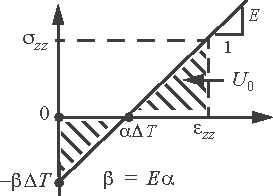
\includegraphics{Figure_5-8.pdf}
\caption{ \label{fig5.8}}
\end{wrapfigure}

\noindent The strain energy density is zero in the unstrained state, since it will be the change in strain energy that is important in subsequent applications. A graphical representation of the strain energy density is obtained in the plot of Hooke's law as shown in figure~\ref{fig5.8}. It is interpreted as the ``area'' between Hooke's law and the strain axis. From the graph the ``area'' is
\begin{align}
U_{0}&=\frac{1}{2} \sigma_{z z}\left(\varepsilon_{z z}-\alpha \Delta T\right)+\frac{1}{2}(-\beta \Delta T)(\alpha \Delta T)\mbox{, or } \nonumber\\
U_{0}&=\frac{E}{2}\left[\left(\varepsilon_{z z}-\alpha \Delta T\right)^{2}-(\alpha \Delta T)^{2}\right]. \label{eq5.35}
\end{align}
Simplification of eq.~(\ref{eq5.35}) reduces it to eq.~(\ref{eq5.34}). The ``area'' represents the work done per unit volume of the stress acting through the strain. The static analog to eq.~(\ref{eq5.30}) is $\sigma_{z z} \delta \varepsilon_{z z}=\delta U_{0}$, where the incremental work per unit volume $\delta W_{0}=\sigma_{z z} \delta \varepsilon_{z z}$. The work done during the deformation is
\begin{align}\label{eq5.36}
W_{0}=\int_{0}^{\varepsilon_{z}} \sigma_{z z} \delta \varepsilon_{z z}=\int_{0}^{\varepsilon_{z}} \delta U_{0}=U_{0}\left(\varepsilon_{z z}\right)-U_{0}(0)=U_{0}\left(\varepsilon_{z z}\right).
\end{align}
That is, the work done per unit volume is equal to the strain-energy-density function, and $W_0$ only depends on the final state of strain and not the strain history.\footnote{Note that reversing the order of application of the mechanical load $\sigma_z$ and thermal load $\Delta T$ changes the ``area'' under the stress-strain plot, which implies $W_0$ is path dependent. See, for example, the discussion in Donaldson (1993, p.~510) and Allen and Haisler (1985, p. 287). However, these authors use eq. (\ref{eq5.34}) for $U_0$.}

Strain energy density functions for a Hookean material subject to a three-dimensional state of strain, including thermal strains, are given by eq. (\ref{eqA.140}) in the appendix. The three-dimensional strain energy density function reduces to eq.~(\ref{eq5.34}) for uniaxial strain if the Poisson effect is neglected.

\subsection{Complementary energy density in uniaxial normal stress}\label{sec5.3.2}

Equation (\ref{eq5.33}) is transformed to a conjugate form by introducing a new function $U_{0}^{*}\left(\sigma_{z z}\right)$ called the complementary-strain-energy density. The transformation was developed by A. M. Legendre. Refer to the~dis\-cussion by Langhaar (1962, p. 120). It is defined by
\begin{align}\label{eq5.37}
U_{0}^{*}\left[\sigma_{z z}\right] \equiv-U_{0}\left[\varepsilon_{z z}\right]+\sigma_{z z} \varepsilon_{z z}.
\end{align}
Take the partial derivative of the complementary-strain-energy density with respect to the normal stress component to get
\begin{align}\label{eq5.38}
\frac{\partial U_{0}^{*}}{\partial \sigma_{z z}}=-\frac{\partial U_{0}}{\partial \varepsilon_{z z}} \frac{\partial \varepsilon_{z z}}{\partial \sigma_{z z}}+\varepsilon_{z z}+\sigma_{z z} \frac{\partial \varepsilon_{z z}}{\partial \sigma_{z z}}=\underbrace{\left[\sigma_{z z}-\left(\frac{\partial U_{0}}{\partial \varepsilon_{z z}}\right)\right]}_{=\,0}\left(\frac{\partial \varepsilon_{z z}}{\partial \sigma_{z z}}\right)+\varepsilon_{z z},
\end{align}
in which the leading term on the right-hand side of eq.~(\ref{eq5.38}) the vanishes by eq.~(\ref{eq5.33}). Hence, complementary-strain-energy density has the property that
\begin{align}\label{eq5.39}
\varepsilon_{z z}=\frac{\partial U_{0}^{*}}{\partial \sigma_{z z}}.
\end{align}
Equation (\ref{eq5.39}) is the conjugate to eq.~(\ref{eq5.33}). Hooke's law for the normal strain is $\varepsilon_{z z}=\left(\sigma_{z z}+\beta \Delta T\right) / E$, which is substituted for the strain in eq.~(\ref{eq5.39}). The result is integrated with respect to the stress to get
\begin{align}\label{eq5.40}
U_{0}^{*}=\int_{-\beta \Delta T}^{\sigma_{z}}\left[\left(\sigma_{z z}+\beta \Delta T\right) / E\right] d \sigma_{z z}=\frac{1}{2 E}\left(\sigma_{z z}+\beta \Delta T\right)^{2}.
\end{align}

\begin{wrapfigure}[10]{L}{132.22pt}
\vspace{-25pt}
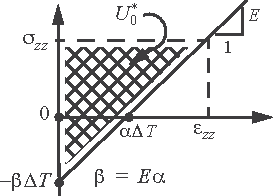
\includegraphics{Figure_5-9.pdf}
\caption{ \label{fig5.9}}
\end{wrapfigure}

\noindent As is shown in figure~\ref{fig5.9}, the complementary-strain-energy density represents the ``area'' between Hooke's law and the stress axis. Expand the last result for the complementary strain energy density to find
\begin{align}\label{eq5.41}
U_{0}^{*}=\frac{1}{2 E}(\sigma_{z z}^{2}+2 \beta \Delta T \sigma_{z z})+\frac{(\alpha \Delta T)^{2}}{2 E}.
\end{align}
The third term in the complementary-strain-energy density above depends only on the change in temperature. This third term in the expression for $U_{0}^{*}$ may be omitted under the assumption of one-way, thermal-mechanical coupling, since the change in temperature is specified independent of the mechanical state. (Refer to the discussion in article \ref{sec3.7.1} on page \pageref{sec3.7.1}.) It is the change in $U_{0}^{*}$ with respect to the stress state that is important in subsequent analyses.


\subsection{Strain energy density in shear}\label{sec5.3.3}

The properties of the strain-energy densities in shear are
\begin{align}\label{eq5.42}
\sigma_{z s}=\frac{\partial U_{0}}{\partial \gamma_{z s}} \quad \gamma_{z s}=\frac{\partial U_{0}^{*}}{\partial \sigma_{z s}}.
\end{align}
Hooke's law relates the shear stress to the shear strain by $\sigma_{z s}=G \gamma_{z s}$, where \textit{G} is the shear modulus of the material. Substituting Hooke's law into eq.~(\ref{eq5.42}) followed by integration, we get the expressions for the strain energy densities as
\begin{align}\label{eq5.43}
U_{0}=\frac{1}{2} G \gamma_{z s}^{2} \quad U_{0}^{*}=\frac{1}{2} \frac{\sigma_{z s}^{2}}{G}.
\end{align}
\begin{wrapfigure}[19]{l}{92.95pt}
\vspace*{-19pt}
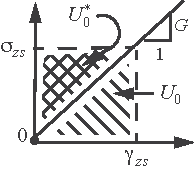
\includegraphics{Figure_5-10.pdf}
\caption{ \label{fig5.10}}
\end{wrapfigure}
\noindent As is shown in figure~\ref{fig5.10}, the strain-energy density is the ``area'' between Hooke's law and the strain axis, and the complementary-strain-energy density is the ``area'' between Hooke's law and the stress axis. Including shear strain $\gamma_{z \zeta}$ and it corresponding shear stress $\sigma_{z \zeta}$, the combined strain energy densities in shear are
\begin{align}\label{eq5.44}
U_{0}=\frac{G}{2}(\gamma_{z s}^{2}+\gamma_{z \zeta}^{2}) \quad U_{0}^{*}=\frac{1}{2 G}(\sigma_{z s}^{2}+\sigma_{z \zeta}^{2}).
\end{align}

\clearpage

\section{Strain energy for extension and bending of a thin-walled bar}\label{sec5.4}

Assuming that the axial normal strain is uniform through the thickness of the wall, we obtain from eq.~(\ref{eq3.30}) on page \pageref{eq3.30} that the axial normal strain is related to the axial displacement $w(z)$, and bending rotations $\phi_{x}(z)$ and $\phi_{y}(z)$,~by
\begin{align}\label{eq5.45}
\varepsilon_{z z}=\frac{d w}{d z}+y(s) \frac{d \phi_{x}}{d z}+x(s) \frac{d \phi_{y}}{d z}.
\end{align}
Substitute eq.~(\ref{eq5.45}) for the normal strain into the strain energy density (\ref{eq5.34}) to get
\begin{align}\label{eq5.46}
U_{0}\left(\varepsilon_{z z}\right)=\frac{E}{2}\left(\frac{d w}{d z}+y(s) \frac{d \phi_{x}}{d z}+x(s) \frac{d \phi_{y}}{d z}\right)^{2}-\beta \Delta T\left(\frac{d w}{d z}+y(s) \frac{d \phi_{x}}{d z}+x(s) \frac{d \phi_{y}}{d z}\right).
\end{align}
The strain energy per unit axial length is defined by $\bar{U}=\int_{c} U_{0}\left(\varepsilon_{z z}\right) t(s) d s$. Substitute eq.~(\ref{eq5.46}) for the strain energy density into the strain energy per unit axial length, and note the geometric properties listed in eqs. (\ref{eq3.74}) and (\ref{eq3.77}) on page \pageref{eq3.77} relative to the centroid, to get
\begin{align}\label{eq5.47}
\bar{U}=\frac{E}{2}\left[A\left(\frac{d w}{d z}\right)^{2}+I_{x x}\left(\frac{d \phi_{x}}{d z}\right)^{2}+I_{y y}\left(\frac{d \phi_{y}}{d z}\right)^{2}+2 I_{x y}\left(\frac{d \phi_{x}}{d z}\right)\left(\frac{d \phi_{y}}{d z}\right)\right]-N_{T}\left(\frac{d w}{d z}\right)-M_{xT}\left(\frac{d \phi_{x}}{d z}\right)-M_{y T}\left(\frac{d \phi_{y}}{d z}\right).
\end{align}
The thermal actions appearing in eq.~(\ref{eq5.47}) are given by eqs. (\ref{eq3.75}) and (\ref{eq3.78}) on page \pageref{eq3.78}.

Assuming that the axial normal stress is uniform through the thickness of the wall, then the axial normal stress is given by eq.~(\ref{eq3.83}) on page \pageref{eq3.83} Substitute eq.~(\ref{eq3.83}) for the normal stress into the expression (\ref{eq5.41}) for the complementary strain energy density to get
\begin{align*}
U_{0}^{*}\left(\sigma_{z z}\right)=&\left(\frac{1}{2 E}\right)\left\{\left[\frac{N+N_{T}}{A}+k \frac{\left(M_{x}+M_{x T}\right)}{I_{x x}} \bar{y}(s)+k \frac{\left(M_{y}+M_{y T}\right)}{I_{y y}} \bar{x}(s)-\beta \Delta T\right]^{2}\right.\\
&+\left.2 \beta \Delta T\left[\frac{N+N_{T}}{A}+k \frac{\left(M_{x}+M_{x T}\right)}{I_{x x}} \bar{y}(s)+k \frac{\left(M_{y}+M_{y T}\right)}{I_{y y}} \bar{x}(s)-\beta \Delta T\right]\right\},
\end{align*}
in which the quadratic term in the temperature change of eq.~(\ref{eq5.41}) is neglected. Expand and simplify the latter expression to find
\begin{align}\label{eq5.48}
U_{0}^{*}\left(\sigma_{z z}\right)=&\frac{1}{2 E}\left\{\left(\frac{N+N_{T}}{A}\right)^{2}+\left[k \frac{\left(M_{x}+M_{x T}\right)}{I_{x x}} \bar{y}(s)\right]^{2}+\left[k \frac{\left(M_{y}+M_{y T}\right)}{I_{y y}} \bar{x}(s)\right]^{2}+2\left(\frac{N+N_{T}}{A}\right)\left(k \frac{M_{x}+M_{x T}}{I_{x x}} \bar{y}(s)\right)\right. \nonumber\\
&+\left.2\left(\frac{N+N_{T}}{A}\right)\left(k \frac{\left(M_{y}+M_{y T}\right)}{I_{y y}} \bar{x}(s)\right)+2\left(k \frac{M_{x}+M_{x T}}{I_{x x}} \bar{y}(s)\right)\left(k \frac{\left(M_{y}+M_{y T}\right)}{I_{y y}} \bar{x}(s)\right)\right\}.
\end{align}
Again, all terms in the simplification of eq.~(\ref{eq5.48}) that contain only the temperature are neglected. The complementary strain energy per unit axial length is defined by $\bar{U}^{*}=\int_{c} U_{0}^{*}\left(\sigma_{z z}\right) t(s) d s$. Substitute eq.~(\ref{eq5.48}) for the complementary strain energy density into the complementary strain energy per unit length. In the evaluation of $\bar{U}^{*}$ we use the definitions given by eqs. (\ref{eq3.74}), (\ref{eq3.81}), and (\ref{eq3.84}) in article \ref{sec3.7.2} on page \pageref{sec3.7.2} to determine the following integrals:
\begin{gather}
\int_{c} \bar{x}(s) t d s=Q_{y}-n_{x} Q_{x}=0 \quad \int_{c} \bar{y}(s) t d s=Q_{x}-n_{y} Q_{y}=0\mbox{, and}\label{eq5.49}\\
\int_{c} \bar{y}^{2} t d s=\frac{I_{x x}}{k} \quad \int_{c} \bar{x}^{2} t d s=\frac{I_{y y}}{k} \quad \int_{c} \bar{x} \bar{y} t d s=\frac{-I_{x y}}{k}.\label{eq5.50}
\end{gather}
The final result for the complementary strain energy per unit length is
\begin{align}\label{eq5.51}
\bar{U}^{*}=\frac{1}{2 E}\left[\frac{\left(N+N_{T}\right)^{2}}{A}+k \frac{\left(M_{x}+M_{x T}\right)^{2}}{I_{x x}}+k \frac{\left(M_{y}+M_{y T}\right)^{2}}{I_{y y}}-2 k I_{x y} \frac{\left(M_{x}+M_{x T}\right)}{I_{x x}} \frac{\left(M_{y}+M_{y T}\right)}{I_{y y}}\right].
\end{align}

\section{Strain energy for shear and torsion of a thin-walled bar}\label{sec5.5}

Consider the strain energy densities due to shear (\ref{eq5.44}). Integrate these strain energy densities over the cross-sectional area to get the strain energies per unit axial length.That is,
\begin{align}\label{eq5.52}
\bar{U}=\frac{1}{2} \int_{c}\left[\int_{-t / 2}^{t / 2} G(\gamma_{z s}^{2}+\gamma_{z \zeta}^{2}) d \zeta\right] d s \quad \bar{U}^{*}=\frac{1}{2} \int_{c}\left[\int_{-t / 2}^{t / 2} \frac{1}{G}(\sigma_{z s}^{2}+\sigma_{z \zeta}^{2}) d \zeta\right] d s.
\end{align}
If we substituted the shear strains $\gamma_{z s}$ and $\gamma_{z \zeta}$ from eq.~(\ref{eq3.31}) on page \pageref{eq3.31} into the strain energy per unit length and performed the integration over the cross section we would get the strain energy function per unit length in the form
\begin{align}\label{eq5.53}
\bar{U}=\bar{U}\left[\psi_{x}, \psi_{y}, \frac{d \phi_{z}}{d z}\right].
\end{align}
Partial derivatives of $\bar{U}$ with respect to the transverse shears and twist per unit length determine the material law for the transverse shear forces and torque. That is,
\begin{align}\label{eq5.54}
V_{x}=\frac{\partial \bar{U}}{\partial \psi_{x}} \quad V_{y}=\frac{\partial \bar{U}}{\partial \psi_{y}} \quad M_{z}=\frac{\partial \bar{U}}{\partial\left(\frac{d \phi_{z}}{d_{z}}\right)}.
\end{align}

The shear stresses enter the definitions of the shear flow $q$, twisting moment resultant $m_{zs}$, and the transverse stress resultant $q_z$, given by eq.~(\ref{eq3.37}) on page \pageref{eq3.37}. For a thin, curved wall we neglect the term $\zeta / R_{s}$ in the factor $\left(1+\zeta / R_{s}\right)$ appearing in the integrand of eq.~(\ref{eq3.37}). It follows that the shear stresses consistent with stress resultant definitions are
\begin{align}\label{eq5.55}
\sigma_{z s}(s, z, \zeta)=\frac{q(s, z)}{t(s)}+\frac{12}{t^{3}(s)} m_{z s}(s, z) \zeta \quad \sigma_{z \zeta}(s, z)=q_{z}(s, z) / t(s).
\end{align}
Substitute eq.~(\ref{eq5.55}) for the stresses in complementary energy per unit length (\ref{eq5.52}), followed by integration through the thickness to get
\begin{align}\label{eq5.56}
\bar{U}^{*}=\frac{1}{2} \int_{c} \frac{q^{2}}{G t} d s+\frac{1}{2} \int_{c} \frac{1}{G}\left[\frac{12}{t^{3}} m_{z s}^{2}+\frac{q_{z}^{2}}{t}\right] d s.
\end{align}

\subsection{Open cross-sectional contour}\label{sec5.5.1}

The shear flow in the first integral on the right-hand side of (\ref{eq5.56}) is given by eq.~(\ref{eq3.98}) on page \pageref{eq3.98}. It is repeated below.
\begin{align}\label{eq5.57}
q(s, z)=-\frac{k}{I_{y y}} V_{x}(z) \bar{Q}_{y}(s)-\frac{k}{I_{x x}} V_{y}(z) \bar{Q}_{x}(s).
\end{align}
\vspace*{5pt}
\clearpage

\noindent Note that the shear flow is directly related to the shear forces and is independent of the torque. To account for the torque, evaluate the second integral on the right-hand side of eq.~(\ref{eq5.56}) for torsion of the open section with the straight contour presented in article \ref{sec3.9} on page \pageref{sec3.9}. From eq.~(\ref{eq3.119}) on page \pageref{eq3.119} these stress resultants are
\begin{align}\label{eq5.58}
m_{z s}=\frac{t^{3}}{6 J}\left(1-\frac{\cosh k s}{\cosh \lambda}\right) M_{z} \quad q_{z}=-2 G t \frac{\sinh k s}{k \cosh \lambda}\left(\frac{d \phi_{z}}{d z}\right) \quad-b / 2 \leq s \leq b / 2,
\end{align}
where
\begin{align*}
\frac{d \phi_{z}}{d z}=\frac{M_{z}}{G J} \quad J=\frac{b t^{3}}{3}\left(1-\frac{\tanh \lambda}{\lambda}\right) \quad k=\frac{2 \sqrt{3}}{t} \quad \lambda=\frac{k b}{2}=\sqrt{3} \frac{b}{t}.
\end{align*}
Substituting the stress resultants $m_{z s}$ and $q_z$ from eq.~(\ref{eq5.58}) into the second integral in the complementary strain energy (\ref{eq5.56}), followed by evaluating the integral, we find
\begin{align}\label{eq5.59}
\frac{1}{2} \int_{c} \frac{1}{G}\left[\frac{12}{t^{3}} m_{z s}^{2}+\frac{q_{z}^{2}}{t}\right] d s=\frac{1}{2 G} \int_{-b / 2}^{b / 2}\left[\frac{12}{t^{3}} m_{z s}^{2}+\frac{q_{z}^{2}}{t}\right] d s=\frac{M_{z}^{2}}{2 G J}.
\end{align}
Hence, the complementary strain energy per unit axial length is
\begin{align}\label{eq5.60}
\bar{U}^{*}=\frac{1}{2} \int_{c} \frac{1}{G t}\left[-\frac{k}{I_{y y}} V_{x}(z) \bar{Q}_{y}(s)-\frac{k}{I_{x x}} V_{y}(z) \bar{Q}_{x}(s)\right]^{2} d s+\frac{M_{z}^{2}}{2 G J}.
\end{align}
We write the eq.~(\ref{eq5.60}) in the form
\begin{align}\label{eq5.61}
\bar{U}^{*}=\frac{1}{2}\left[c_{x x} V_{x}^{2}+2 c_{x y} V_{x} V_{y}+c_{y y} V_{y}^{2}\right]+\frac{M_{z}^{2}}{2 G J},
\end{align}
where $c_{x x}, c_{x y}, c_{y x}$, and $c_{y y}$ are the flexibility influence coefficients for the cross section of the bar given by
\begin{align}\label{eq5.62}
c_{x x}=\left(\frac{k}{I_{y y}}\right)^{2} \int_{c} \frac{\left[\bar{Q}_{y}(s)\right]^{2}}{G t} d s\quad c_{x y}=c_{y x}=\frac{k^{2}}{I_{x x} I_{y y}} \int_{c} \frac{\left[\bar{Q}_{x}(s) \bar{Q}_{y}(s)\right]}{G t} d s\quad c_{y y}=\left(\frac{k}{I_{x x}}\right)^{2} \int_{c} \frac{\left[\bar{Q}_{x}(s)\right]^{2}}{G t} d s.
\end{align}

\subsection{Closed cross-sectional contour}\label{sec5.5.2}

The shear flow for the closed cross-sectional contour is directly related to the shear forces and the torque resolved at the shear center. Equation (\ref{eq3.163}) on page \pageref{eq3.163} is
\begin{align*}
q(s, z)=\frac{M_{z}(z)}{2 A_{c}}-F_{x}(s) V_{x}(z)-F_{y}(s) V_{y}(z),
\end{align*}
where the shear flow distribution functions $F_{x}(s)$ and $F_{y}(s)$ are determined from eqs. (\ref{eq3.151}) and (\ref{eq3.164}) on page \pageref{eq3.164}. For the closed section the stress resultants $m_{z s}$ and $q z$ are assumed negligible with respect to the shear flow $q$. Consequently, in the complementary strain energy per unit axial length (\ref{eq5.56}) the second integral on the right-hand side is neglected with respect to the first integral on the right-hand side. The complementary strain energy per unit axial length is then given by
\begin{align}\label{eq5.63}
\bar{U}^{*}=\frac{1}{2} \int_{c}\frac{1}{G t}\left[\frac{M_{z}(z)}{2 A_{c}}-F_{x}(s) V_{x}(z)-F_{y}(s) V_{y}(z)\right]^{2} d s.
\end{align}
Expand the integrand of latter equation and write it as
\begin{align}\label{eq5.64}
\bar{U}^{*}=\frac{1}{2}\left[c_{x x} V_{x}^{2}+c_{y y} V_{y}^{2}+c_{z z} M_{z}^{2}+2 c_{x z} V_{x} M_{z}+2 c_{y z} V_{y} M_{z}+2 c_{x y} V_{x} V_{y}\right].
\end{align}
The flexibility influence coefficients for the closed cross-sectional contour are
\begin{gather}
c_{x x}=\oint\frac{F_{x}^{2}}{G t} d s \quad c_{y y}=\oint \frac{F_{y}^{2}}{G t} d s \quad c_{z z}=\frac{1}{4 A_{c}^{2}} \oint \frac{d s}{G t}=\frac{1}{G J}\mbox{, and}\label{eq5.65}\\
c_{xz}=c_{zx}=\left(\frac{1}{2A_c}\right)\int_c\frac{F_x}{Gt}ds=0\quad c_{yz}=c_{zy}=\left(\frac{1}{2A_c}\right)\int_c\frac{F_y}{Gt}ds=0\quad
c_{xy}=c_{yx}=\oint\frac{F_xF_y}{Gt}ds.\label{eq5.66}
\end{gather}
The torsion constant \textit{J} for a single-cell cross section is given by eq.~(\ref{eq3.160}) on page \pageref{eq3.160}. Influence coefficients $c_{x z}=c_{y z}=0$, since the shear flow distribution functions $F_{x}(s)$ and $F_{y}(s)$ are defined with respect to the shear center. (Refer to eq.~(\ref{eq3.151}) and eq.~(\ref{eq3.164}).)

\subsection{Material law for transverse shear and torsion}\label{sec5.5.3}

The relation between the strain energy densities in shear is analogous to the one for normal stress and strain (\ref{eq5.37}). This relation is
\begin{align}\label{eq5.67}
U_{0}^{*}\left[\sigma_{z s}\right] \equiv-U_{0}\left[\gamma_{z s}, \gamma_{z \zeta}\right]+\sigma_{z s} \gamma_{z s}+\sigma_{z \zeta} \gamma_{z \zeta}.
\end{align}
Integrate eq.~(\ref{eq5.67}) over the cross-sectional area to get
\begin{align}\label{eq5.68}
\underbrace{\int_{c}\left[\int_{-t / 2}^{t / 2} U_{0}^{*}\left[\sigma_{z s}\right] d \zeta\right] d s}_{\bar{U}^{*}\left[V_{x}, V_{y},\, M_{z}\right]}= -\underbrace{\int_{c}\left[\int_{-t / 2}^{t/2} U_{0}\left[\gamma_{z s}, \gamma_{z \zeta}\right] d \zeta\right] d s}_{\bar{U}\left[\psi_{x}, \psi_{y}, \frac{d \phi}{d z} z\right]}+ \underbrace{\int_c\left[\int_{-t / 2}^{t / 2}\left(\sigma_{z s} \gamma_{z s}+\sigma_{z \zeta} \gamma_{z \zeta}\right) d \zeta\right] d s}_{I}.
\end{align}
Substitute (\ref{eq5.55}) for the stresses, and eq.~(\ref{eq3.31}) on page \pageref{eq3.31} for the strains, in the second integral labeled \textit{I} on the right-hand side of eq.~(\ref{eq5.68}). After integration over the thickness the integral \textit{I} is
\begin{align}\label{eq5.69}
I=\int_{c}\left[q\left(-\psi_{x} \sin \theta+\psi_{y} \cos \theta+r_{n} s \frac{d \phi_{z}}{d z}\right)+m_{z s} \frac{d \phi_{z}}{d z}+q_{z}\left(\psi_{x} \cos \theta+\psi_{y} \sin \theta-r_{t} \frac{d \phi_{z}}{d z}\right)\right] d s.
\end{align}
Rearrange the integrand in eq.~(\ref{eq5.69}) to
\begin{align}\label{eq5.70}
I=\left[\int_{c}\left(-q \sin \theta+q_{z} \cos \theta\right) d s\right] \psi_{x}+\left[\int_{c}\left(q \cos \theta+q_{z} \sin \theta\right) d s\right] \psi_{y}+\left[\int_{c}\left(r_{n} q+m_{z s}-r_{t} q_{z}\right) d s\right] \frac{d \phi_{z}}{d z}.
\end{align}
From eq.~(\ref{eq3.40}) on page \pageref{eq3.40} recognize that the coefficient of shear $\psi_{x}$ is the shear force $V_x$, the coefficient of shear $\psi_{y}$ is the shear force $V_y$, and the coefficient of the twist per unit length is the torque $M_z$. Hence, the integral $I$ is given by
\begin{align}\label{eq5.71}
I=\int_{c}\left[\int_{-t / 2}^{t / 2}\left(\sigma_{z s} \gamma_{z s}+\sigma_{z \zeta} \gamma_{z \zeta}\right) d \zeta\right] d s=V_{x} \psi_{x x}+V_{y} \psi_{y y}+M_{z} \frac{d \phi_{z}}{d z}.
\end{align}
The relation between the shear strain energies per unit axial length in eq.~(\ref{eq5.68}) becomes
\begin{align}\label{eq5.72}
\bar{U}^{*}\left[V_{x}, V_{y}, M_{z}\right]=-\bar{U}\left[\psi_{x}, \psi_{y} \frac{d \phi_{z}}{d z}\right]+V_{x} \psi_{x}+V_{y} \psi_{y}+M_{z} \frac{d \phi_{z}}{d z}.
\end{align}
Take the partial derivative of (\ref{eq5.72}) with respect to the shear force $V_x$ as follows:
\begin{align}\label{eq5.73}
\frac{\partial \bar{U}^{*}}{\partial V_{x}}=-\frac{\partial \bar{U}}{\partial \psi_{x}} \frac{\partial \psi_{x}}{\partial V_{x}}+\psi_{x}+V_{x} \frac{\partial \psi_{x}}{\partial V_{x}}=\left(V_{x}-\frac{\partial \bar{U}}{\partial \psi_{x}}\right)\left(\frac{\partial \psi_{x}}{\partial V_{x}}\right)+\psi_{x}.
\end{align}
The term $V_{x}-\partial \bar{U} / \partial \psi_{x}=0$ in eq.~(\ref{eq5.73}) since it is the elastic material law for the shear force given by eq.~(\ref{eq5.54}). Consequently, eq.~(\ref{eq5.73}) leads to the material law for shear $\psi_{x}$
\begin{align}\label{eq5.74}
\frac{\partial \bar{U}^{*}}{\partial V_{x}}=\psi_{x}.
\end{align}
Following steps similar to those used in eqs. (\ref{eq5.72}) to (\ref{eq5.74}) leads to the additional material laws
\begin{align}\label{eq5.75}
\frac{\partial \bar{U}^{*}}{\partial V_{y}}=\psi_{y}\mbox{ and }\frac{\partial \bar{U}^{*}}{\partial M_{z}}=\frac{d \phi_z}{d z}.
\end{align}

\vspace*{-1pc}

Substitute the complementary strain energy from either eq.~(\ref{eq5.61}) or (\ref{eq5.64}) into eqs. (\ref{eq5.74}) and (\ref{eq5.75}) to obtain the material law governing the transverse shears and the twist per unit length. Since the expressions for the complementary strain energy per unit axial length with respect to the shear center are the same for the open contour (\ref{eq5.61}) and the closed contour (\ref{eq5.64}), the material law in both cases is
\begin{align}\label{eq5.76}
\left[\begin{array}{@{}c@{}}\psi_{x} \\[2pt] \psi_{y} \\[4pt] \frac{d \phi_{z}}{d_{z}}\end{array}\right]=\left[\begin{array}{@{}ccc@{}}c_{x x} & c_{x y} & 0 \\c_{x y} & c_{y y} & 0 \\0 & 0 & 1 /(G J)\end{array}\right]\left[\begin{array}{@{}c@{}}V_{x} \\V_{y} \\M_{z}\end{array}\right].
\end{align}
Assume we can invert the material law (\ref{eq5.76}) and write it as
\begin{align}\label{eq5.77}
\left[\begin{array}{@{}c@{}}V_{x} \\V_{y} \\M_{z}\end{array}\right]=\left[\begin{array}{@{}ccc@{}}s_{x x} & s_{x y} & 0 \\s_{x y} & s_{y y} & 0 \\0 & 0 & G J\end{array}\right]\left[\begin{array}{@{}c@{}}\psi_{x} \\\psi_{y} \\\phi_{z}^{\prime}\end{array}\right],
\end{align}
where
\begin{align}\label{eq5.78}
\left[s_{x x}, s_{y y}, s_{x y}\right]=\left[c_{y y}, c_{x x},-c_{x y}\right] /\left(c_{x x} c_{y y}-c_{x y}^{2}\right).
\end{align}
The strain energy per unit axial length in shear and torsion is
\begin{align}\label{eq5.79}
\bar{U}=\frac{1}{2}\left[s_{x x} \psi_{x}^{2}+2 s_{x y} \psi_{x} \psi_{y}+s_{y y} \psi_{y}^{2}+G J\left(\frac{d \phi_{z}}{d z}\right)^{2}\right].
\end{align}

\section{Total strain energy expressions for a thin-walled bar}\label{sec5.6}

The total strain energy is obtained from strain energy per unit axial length by integration with respect to axial coordinate $z$, $0 \leq z \leq L$, where $L$ is the length of the bar. The total strain energy is written as
\begin{align}\label{eq5.80}
U=U_{\varepsilon}+U_{\gamma},
\end{align}
where the strain energy obtained from axial normal strain $\varepsilon_{z z}$ is denoted by $U_{\varepsilon}$, and the strain energy obtained from shear strains $\gamma_{z s}$ and $\gamma_{z \xi}$ is denoted by $U_{\gamma}$. From eqs. (\ref{eq5.47}) and (\ref{eq5.79}) these strain energies are\pagebreak
\begin{align}\label{eq5.81}
U_{\varepsilon}=\int_{0}^{L}&\left\{\frac{E}{2}\left[A\left(\frac{d w}{d z}\right)^{2}+I_{x x}\left(\frac{d \phi_{x}}{d z}\right)^{2}+I_{y y}\left(\frac{d \phi_{y}}{d z}\right)^{2}+2 I_{x y}\left(\frac{d \phi_{x}}{d z}\right)\left(\frac{d \phi_{y}}{d z}\right)\right]\right.\nonumber\\
&\qquad\left.-N_{T}\left(\frac{d w}{d z}\right)-M_{x T}\left(\frac{d \phi_{x}}{d z}\right)-M_{y T}\left(\frac{d \phi_{y}}{d z}\right)\right\} d z,
\end{align}
and
\begin{align}\label{eq5.82}
U_{\gamma}=\frac{1}{2} \int^L_0\left[s_{x x} \psi_{x}^{2}+2 s_{x y} \psi_{x} \psi_{y}+s_{y y} \psi_{y}^{2}+G J\left(\frac{d \phi_{z}}{d z}\right)^{2}\right] d z.
\end{align}
The stiffness coefficients in eq.~(\ref{eq5.82}) are computed from the compliance coefficients as shown in eq.~(\ref{eq5.78}).

The total complementary strain energy is written as
\begin{align}\label{eq5.83}
U^{*}=U_{\sigma}^{*}+U_{\tau}^{*},
\end{align}
where the complementary strain energy obtained from axial normal stress $\sigma_{z z}$ is denoted by $U_{\sigma}^{*}$, and the complementary strain energy obtained from shear stresses $\sigma_{z s}$ and $\sigma_{z \zeta}$ is denoted by $U_{\tau}^{*}$. From eqs. (\ref{eq5.51}) and (\ref{eq5.61}) these complementary strain energies are
\begin{align}\label{eq5.84}
U_{\sigma}^{*}=\frac{1}{2 E} \int_{0}^{L}\left[\frac{\left(N+N_{T}\right)^{2}}{A}+k \frac{\left(M_{x}+M_{x T}\right)^{2}}{I_{x x}}+k \frac{\left(M_{y}+M_{y T}\right)^{2}}{I_{y y}}-2 k I_{x y} \frac{\left(M_{x}+M_{x T}\right)}{I_{x x}} \frac{\left(M_{y}+M_{y T}\right)}{I_{y y}}\right] d z,
\end{align}
and
\begin{align}\label{eq5.85}
U_{\tau}^{*}=\frac{1}{2} \int_{0}^{L}\left[c_{x x} V_{x}^{2}+2 c_{x y} V_{x} V_{y}+c_{y y} V_{y}^{2}+\frac{M_{z}^{2}}{G J}\right] d z.
\end{align}
The compliance coefficients in eq.~(\ref{eq5.85}) are determined by eq.~(\ref{eq5.62}) for the open contour and by eqs. (\ref{eq5.65}) and (\ref{eq5.66}) for the closed contour.

\section{Castigliano's first theorem}\label{sec5.7}

The work function can be written in terms of the generalized displacements and stiffness influence coefficients by substituting $n=2$ in eq.~(\ref{eq5.10}), then substituting the result for the generalized forces into the work eq.~(\ref{eq5.5}). The result is
\begin{align}\label{eq5.86}
W=\left(\frac{1}{2}\right)\left(k_{11} q_{1}^{2}+2 k_{12} q_{1} q_{2}+k_{22} q_{2}^{2}\right).
\end{align}
Take the partial derivative of the work function with respect to $q_1$ and $q_2$ to get
\begin{align*}
\frac{\partial W}{\partial q_{1}}=k_{11} q_{1}+k_{12} q_{2} \quad \frac{\partial W}{\partial q_{2}}=k_{12} q_{1}+k_{22} q_{2}.
\end{align*}
Comparing these results for the partial derivatives of $W$ to the eq.~(\ref{eq5.10}) for $n=2$, we find
\begin{align}\label{eq5.87}
Q_{1}=\frac{\partial W}{\partial q_{1}} \quad Q_{2}=\frac{\partial W}{\partial q_{2}}.
\end{align}
That is, the partial derivative of the work function with respect to a displacement equals the corresponding force. Equation (\ref{eq5.87}) yields the stiffness law, and it is the conjugate to eq.~(\ref{eq5.8}) that yields the compliance law.

For adiabatic deformation of a Hookean material the first law of thermodynamics shows that the work done per unit volume is equal to the strain energy density. Refer to eq.~(\ref{eq5.36}) on page \pageref{eq5.36}. For the body composed of a Hookean material, we take the work done by the external loads equal to the strain energy of the entire body. Then $W=U$ in eq.~(\ref{eq5.87}), which leads to Castigliano's first theorem in terms of generalized displacements and forces as follows:

\begin{framed}
\noindent\textbf{Castigliano's first theorem}\\
\hspace*{-10pt}\rule{37.45pc}{2pt}
If the strain energy of an elastic structure is expressed in terms of the independent generalized displacement components $q_{i}$, $i=1,2, \ldots, n$, in the direction of the prescribed generalized point forces $Q_{1}, Q_{2}, \ldots Q_{n}$, then the first partial derivative of the strain energy with respect to the displacement $q_{i}$ is equal to the corresponding force $Q_{i}$ or\vspace*{-4pt}
\begin{align*}
Q_{i}=\frac{\partial U}{\partial q_{i}} \quad i=1,2, \ldots, n
\end{align*}
\vspace*{-13pt}
\end{framed}

For the thin-walled bar the strain energy $U$ is given by eqs. (\ref{eq5.80}) to (\ref{eq5.82}), and it has the form
\begin{align*}
U=\int_{0}^{L} \bar{U}(w^{\prime}, \phi_{x}^{\prime}, \phi_{y}^{\prime}, \phi_{z}^{\prime}, \psi_{x}, \psi_{y}) d z.
\end{align*}
The prime indicates ordinary derivative with respect to coordinate $z$ \big(e.g. $w^{\prime}=\frac{d w}{d z}$\big), and the averaged shears from eq.~(\ref{eq3.32}) on page \pageref{eq3.32} are repeated below.
\begin{align*}
\psi_{x}(z)=\frac{d u}{d z}+\phi_{y}(z) \quad \psi_{y}(z)=\frac{d v}{d z}+\phi_{x}(z).
\end{align*}
The procedure in the application of the first theorem to structural analysis is to assume functions for the displacement components $u(z), v(z)$, and $w(z)$ and rotations $\phi_{x}(z), \phi_{y}(z)$, and $\phi_{z}(z)$ that satisfy the three conditions below.
\begin{enumerate}
\item[1.] The displacement and rotations must be continuous functions of the coordinate $z$, so that their derivatives with respect to the coordinate, or strains, exist and are integrable over the domain of the bar.

\item[2.] The displacement and rotations must satisfy any prescribed conditions at the boundaries $z = 0$ and $z = L$.

\item[3.] The displacement and rotation functions are selected such that they equate to the generalized displacements $q_{i}$, $i=1,2, \ldots, n$, at their defined points of application.
\end{enumerate}

Displacement and rotation functions that satisfy continuity conditions and prescribed displacement boundary conditions are said to be \textbf{kinematically admissible}. Kinematically admissible displacements lead to a compatible deformation. Compatibility of a deformable body means the displacements are continuous and single-valued (i.e., no gaps or overlaps of material result in the deformed state). \textbf{Castigliano's first theorem is a condition of equilibrium consistent with the assumed kinematically admissible displacements}.

\clearpage

\begin{example}[Response of cantilever beam by Castigliano's first theorem]\label{ex5.1}\setcounter{equation}{0}\def\theequation{\alph{equation}}The cantilever beam shown in figure~\ref{fig5.11} is subject to a vertical displacement $q_1$ and a clockwise ration $q_2$ at its tip, and a uniform thermal moment $M_{xT}$ along its length. The cross section is symmetric with respect to the \textit{y-z} plane.

\processfigure{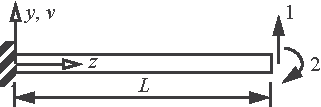
\includegraphics{Figure_5-11.pdf}}{\caption{Cantilever beam subject to a temperature gradient and end loads.}\label{fig5.11}}

\noindent Assume a kinematically admissible displacement and bending rotation as
\begin{align}\label{ex5.1a}
v(z)=q_{1}(z / L) \quad \phi_{x}(z)=q_{2}(z / L) \quad 0 \leq z \leq L.
\end{align}
Continuous and differentiable functions for the generalized displacements are ensured by employing polynomial functions in coordinate $z$. Also, assumptions ({\bf\ref{ex5.1a}}) satisfy the prescribed end conditions $v(0)=0$ and $\phi_{x}(0)=0$. Therefore, assumptions ({\bf\ref{ex5.1a}}) satisfy the conditions of kinematic admissibility. The strain energy reduces to a function generalized displacements $q_1$ and $q_2$. For this example the expression for the strain energy from (\ref{eq5.81}) and\break (\ref{eq5.82}) is
\begin{align}\label{ex5.1b}
U=\int_{0}^{L} \bar{U}\left[\phi_{x}^{\prime}, \psi_{y}\right] d z\mbox{ where }\bar{U}\left[\phi_{x}^{\prime}, \psi_{y}\right]=\frac{1}{2} E I_{x x}\left(\phi_{x}^{\prime}\right)^{2}-M_{x T}\left(\phi_{x}^{\prime}\right)+\frac{1}{2} s_{y y} \psi_{y}^{2}.
\end{align}
The derivatives of the functions in ({\bf\ref{ex5.1a}}) with respect to $z$, and the evaluation of the transverse shear strain are
\begin{align}\label{ex5.1c}
v^{\prime}(z)=q_{1} / L \quad \phi_{x}^{\prime}(z)=q_{2} / L \quad \psi_{y}(z)=q_{1} / L+q_{2}(z / L).
\end{align}
Substitute eq. ({\bf\ref{ex5.1c}}) into eq. ({\bf\ref{ex5.1b}}) to get
\begin{align}\label{ex5.1d}
\bar{U}=\frac{E I_{x x}}{2 L^{2}} q_{2}^{2}+\frac{s_{y y}}{2}\left(\frac{q_{1}}{L}+\frac{q_{2}}{L} z\right)^{2}-\frac{M_{x T}}{L} q_{2}.
\end{align}
The definite integral of eq. ({\bf\ref{ex5.1d}}) over the length of beam yields the discrete form of the strain energy ({\bf\ref{ex5.1b}}). The result~is
\begin{align}\label{ex5.1e}
U\left(q_{1}, q_{2}\right)=\frac{E I_{x x}}{2 L} q_{2}^{2}+\frac{s_{y y}}{2 L} q_{1}^{2}+\frac{s_{y y}}{2} q_{1} q_{2}+\frac{s_{y y} L}{6} q_{2}^{2}-M_{x T}\hspace*{1pt}q_{2}.
\end{align}
The strain energy expression in eq. ({\bf\ref{ex5.1b}}) is called a \textbf{functional} because its value is determined by the functions $\phi_{x}(z)$ and $\psi_{y}(z)$. Assumption ({\bf\ref{ex5.1a}}) results in a strain energy function given by eq. ({\bf\ref{ex5.1e}}) where the generalized displacements $q_{1}$ and $q_{2}$ are the independent variables. The generalized forces $Q_{1}$ and $Q_{2}$ corresponding to $q_{1}$ and $q_{2}$, respectively, are determined by Castigliano's first theorem. That is,
\begin{align}\label{ex5.1f}
Q_{1}=\frac{\partial U}{\partial q_{1}}\mbox{ and }Q_{2}=\frac{\partial U}{\partial q_{2}}.
\end{align}
Take the partial derivatives of eq. ({\bf\ref{ex5.1e}}) with respect to $q_{1}$ and $q_{2}$ to find
\begin{align}\label{ex5.1g}
Q_{1}=\frac{s_{y y}}{L} q_{1}+\frac{s_{y y}}{2} q_{2}\mbox{ and }Q_{2}=\frac{s_{y y}}{2} q_{1}+\left(\frac{E I_{x x}}{L}+\frac{L s_{y y}}{3}\right) q_{2}-M_{x T}.
\end{align}
\vspace*{5pt}
\clearpage

\noindent The expressions in eq. ({\bf\ref{ex5.1g}}) are written in the matrix form
\begin{align}\label{ex5.1h}
\left[\begin{array}{@{}l@{}}Q_{1} \\Q_{2}\end{array}\right]=\left[\begin{array}{@{}cc@{}}\frac{s_{y y}}{L} & \frac{s_{y y}}{2} \\\frac{s_{y y}}{2} & \frac{E I_{x x}}{L}+\frac{L s_{y y}}{3}\end{array}\right]\left[\begin{array}{@{}l@{}}q_{1} \\q_{2}\end{array}\right]-\left[\begin{array}{@{}l@{}}0 \\1\end{array}\right] M_{x T}.
\end{align}
The elements of the 2X2 stiffness matrix in eq. ({\bf\ref{ex5.1h}}) are the stiffness influence coefficients. Also note than the stiffness matrix is symmetric.

From eq.~(\ref{eq3.79}) Hooke's law for the bending moment is
\begin{align}\label{ex5.1i}
M_{x}=E I_{x x} \phi_{x}^{\prime}(z)-M_{x T},
\end{align}
and from eq.~(\ref{eq5.77}) the material law for the transverse shear force $i$
\begin{align}\label{ex5.1j}
V_{y}=s_{y y} \psi_{y}.
\end{align}
Substitute $\phi_{x}^{\prime}$ and $\psi_{y}$ from eq. ({\bf\ref{ex5.1c}}) into eqs. ({\bf\ref{ex5.1i}}) and ({\bf\ref{ex5.1j}}) to get
\begin{align}\label{ex5.1k}
M_{x}=E I_{x x}\left(q_{2} / L\right)-M_{x T}\mbox{ and }V_{y}=s_{y y}\left(q_{1} / L+q_{2}(z / L)\right).
\end{align}
Equilibrium differential equations (\ref{eq3.54}) and (\ref{eq3.55}) are
\begin{align}\label{ex5.1l}
\frac{d V_{y}}{d z}=0\mbox{ and }\frac{d M_{x}}{d z}-V_{y}=0\mbox{ for }0<z<L.
\end{align}
Substitute the bending moment and shear force from eq. ({\bf\ref{ex5.1k}}) into eq. ({\bf\ref{ex5.1l}}) to get
\begin{align}\label{ex5.1m}
\frac{d V_{y}}{d z}=\frac{s_{y y}}{L} q_{2} \neq 0\mbox{ and }\frac{d M_{x}}{d z}-V_{y}=0-\left(\frac{s_{y y}}{L} q_{2} z+c\right) \neq 0,
\end{align}
where $c$ denotes a constant of integration for the shear force. The differential equations are not satisfied for the assumption in eq. ({\bf\ref{ex5.1a}}). Of all the possible kinematically admissible displacement functions those given by ({\bf\ref{ex5.1a}}) lead to an approximate equilibrium solution but not the exact equilibrium solution.
\end{example}\setcounter{equation}{87}

\vspace*{-15pt}

\section{Castigliano's second theorem}\label{sec5.8}

The generalized displacements from Hooke's law in eq.~(\ref{eq5.3}) are substituted into the work eq.~(\ref{eq5.5}) to express the work function as
\begin{align*}
W=\left(\frac{1}{2}\right)\big(c_{11} Q_{1}^{2}+c_{12} Q_{1} Q_{2}+c_{21} Q_{2} Q_{1}+c_{22} Q_{2}^{2}\big).
\end{align*}
Take the partial derivative of the work function with respect to $Q_1$ and $Q_2$ to get
\begin{align*}
\frac{\partial W}{\partial Q_{1}}=c_{11} Q_{1}+c_{12} Q_{2} \quad \frac{\partial W}{\partial Q_{2}}=c_{12} Q_{1}+c_{22} Q_{2}.
\end{align*}
Comparing these results for the partial derivatives of \textit{W} to the two equations (\ref{eq5.3}), we find
\begin{align}\label{eq5.88}
q_{1}=\frac{\partial W}{\partial Q_{1}}\mbox{ and }q_{2}=\frac{\partial W}{\partial Q_{2}}.
\end{align}
If the work function is written in terms of the forces and flexibility influence coefficients, then partial derivatives of the work with respect to a force equals the corresponding displacement. The work done on a Hookean body is equal to the change in energy stored due to elastic deformation. We use the complementary strain energy $U^{*}$ in this case to represent the change in energy since $U^{*}=0$ in the reference state. Hence, set $W=U^{*}$, and we arrive at Castigliano's second theorem in terms of generalized displacements and forces, which is as follows:

\begin{framed}
\noindent\textbf{Castigliano's second theorem}\\
\hspace*{-10pt}\rule{37.45pc}{2pt}
If an elastic structure is mounted such that rigid body displacements are impossible and certain generalized point forces $Q_{1}, Q_{2}, \ldots, Q_{n}$ act on the structure, in addition to distributed loads and thermal strains, the displacement component $q_{i}$, $i=1,2, \ldots, n$ of the point of application of force $Q_{i}$ in the direction of $Q_{i}$ is determined by the equation\vspace*{-8pt}
\begin{align*}
q_{i}=\frac{\partial U^{*}}{\partial Q_{i}}.
\end{align*}\vspace*{-16pt}
\end{framed}\vspace*{-7pt}

For a thin-walled bar the complementary strain energy given by eqs. (\ref{eq5.83}) to (\ref{eq5.85}) has the form
\begin{align}\label{eq5.89}
U^{*}=\int_{0}^{L} \bar{U}^{*}\left(V_{x}, V_{y}, N, M_{x}, M_{y}, M_{z}\right) d z.
\end{align}
The procedure in the application of the second theorem to the analysis of thin-walled bars is to assume functions in the axial coordinate $z$ for the bar resultants $V_{x}, V_{y}, N, M_{x}, M_{y}$, and $M_{z}$, that satisfy the three conditions below.
\begin{enumerate}
\item[1.] The bar resultants must be represented by functions of the Cartesian coordinates that satisfy the differential equations of equilibrium of article \ref{sec3.6.1} on page \pageref{sec3.6.1} for $0<z<L$.

\item[2.] The functions for the bar resultants must satisfy their prescribed values on the boundaries at $z = 0$ and $z = L$.

\item[3.] The functions for the bar resultants must contain the generalized forces $Q_{i}$, $i=1,2, \ldots, n$, as parameters.
\end{enumerate}

Functions for the bar resultants that satisfy the differential equations of equilibrium and prescribed force boundary conditions are said to be \textbf{statically admissible. Castigliano's second theorem is the condition of compatibility for the statically admissible bar resultants.} Compatibility of a deformable body means the displacements are continuous and single-valued (i.e., no gaps or overlaps of material result in the deformed state). Castigliano's second theorem is useful in determining displacements of a structure.

\vspace*{-10pt}

\begin{example}[Response of the cantilever beam by Castigliano's second theorem]\label{ex5.2}\setcounter{equation}{0}\def\theequation{\alph{equation}}

\begin{wrapfigure}[7]{R}{107pt}
\vspace*{-19pt}
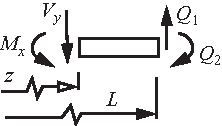
\includegraphics{Figure_5-12.pdf}
\caption{Free body diagram of the beam. \label{fig5.12}}
\end{wrapfigure}

\vspace*{-20pt}

\noindent Consider the cantilever beam in example \ref{ex5.1} on page \pageref{ex5.1} again. Take the end loads $Q_1$ and $Q_2$ to be specified, and use Castigliano's second theorem to determine the corresponding displacements $q_1$ and $q_2$. We note that the beam in this example is statically determinate. From equilibrium of the free body diagram shown in figure~\ref{fig5.12} the statically admissible internal actions are.
\begin{align}\label{ex5.2a}
V_{y}=Q_{1} \quad M_{x}=Q_{2}-Q_{1}(L-z) \quad 0 \leq z \leq L.
\end{align}
The complementary strain energy from (\ref{eq5.84}) and (\ref{eq5.85}) is
\begin{align}\label{ex5.2b}
U^{*}=\int_{0}^{L} \bar{U}^{*}\left[V_{y}, M_{x}\right] d z\mbox{, where }\bar{U}^{*}\left[V_{y}, M_{x}\right]=\frac{1}{2} c_{y y} V_{y}^{2}+\frac{1}{2 E I_{x x}}\left(M_{x}+M_{x T}\right)^{2}.
\end{align}

\clearpage

%\vspace*{-1pc}\clearpage
%\begin{wrapfigure}[9]{R}{107pt}
%%\vspace*{-19pt}
%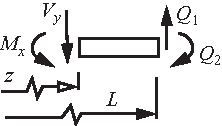
\includegraphics{Figure_5-12.pdf}
%\caption{Free body diagram of the beam. \label{fig5.12}}
%\end{wrapfigure}

Substitute the shear force and bending moment from eq. ({\bf\ref{ex5.2a}}) into the complementary strain energy per unit axial length given in eq. ({\bf\ref{ex5.2b}}) to get
\begin{align}\label{ex5.2c}
\bar{U}^{*}=\frac{c_{y y}}{2} Q_{1}^{2}+\frac{\left[Q_{2}-(L-z) Q_{1}+M_{x T}\right]^{2}}{2 E I_{x x}}.
\end{align}
Integrate eq. (\textbf{c}) over the length of the beam to find the complementary strain energy~as
\begin{align}
U^{*}=\left(\frac{c_{y y} L}{2}+\frac{L^{3}}{6 E I_{x x}}\right) Q_{1}^{2}-\frac{L^{2}}{2 E I_{x x}} Q_{1} Q_{2}+\frac{L}{2 E I_{x x}} Q_{2}^{2}-\frac{L^{2}}{2 E I_{x x}} M_{x T} Q_{1} +\frac{L}{E I_{x x}} M_{x T} Q_{2}+\frac{L M_{x T}^{2}}{2 E I_{x x}}. \label{ex5.2d}
\end{align}
The statically admissible functions assumed in eq. ({\bf\ref{ex5.2a}}) transform the complementary strain energy functional given by eq. ({\bf\ref{ex5.2b}}) to a function of the independent variables $Q_{1}$ and $Q_{2}$ in eq. ({\bf\ref{ex5.2d}}). Castiglinao's second theorem determines the generalized displacements $q_{1}$ and $q_{2}$ corresponding to the generalized forces $Q_{1}$ and $Q_{2}$. That is,
\begin{align}\label{ex5.2e}
q_{1}=\frac{\partial {U}^{*}}{\partial Q_{1}}\mbox{ and }q_{2}=\frac{\partial {U}^{*}}{\partial Q_{2}}.
\end{align}
Substitute the complementary strain energy ({\bf\ref{ex5.2d}}) into Castigliano's second theorem ({\bf\ref{ex5.2e}}) to get
\begin{gather}
q_{1}=\left(c_{y y} L+\frac{L^{3}}{3 E I_{x x}}\right) Q_{1}-\frac{L^{2}}{3 E I_{x x}} Q_{2}-\frac{L^{2}}{2 E I_{x x}} M_{x T}\mbox{, and}\label{ex5.2f}\\
q_{2}=-\frac{L^{2}}{E I_{x x}} Q_{1}+\frac{L}{E I_{x x}} Q_{2}+\frac{L}{E I_{x x}} M_{x T}.\label{ex5.2g}
\end{gather}
Equations ({\bf\ref{ex5.2f}}) and ({\bf\ref{ex5.2g}}) are written in the matrix form as
\begin{align}\label{ex5.2h}
\left[\begin{array}{@{}l@{}}q_{1} \\q_{2}\end{array}\right]=\left[\begin{array}{@{}cc@{}}c_{y y} L+\displaystyle\frac{L^{3}}{3 E I_{x x}} & \displaystyle-\frac{L^{2}}{2 E I_{x x}} \\[8pt]\displaystyle-\frac{L^{2}}{2 E I_{x x}} & \displaystyle\frac{L}{E I_{x x}}\end{array}\right]\left[\begin{array}{@{}l@{}}Q_{1} \\Q_{2}\end{array}\right]+\left[\begin{array}{@{}c@{}}\displaystyle-\frac{L^{2}}{2 E I_{x x}} \\[10pt]
\displaystyle\frac{L}{E I_{x x}}\end{array}\right] M_{x T}.
\end{align}
The elements of the 2X2 compliance matrix in eq. ({\bf\ref{ex5.2h}}) are the flexibility influence coefficients. Also note that the compliance matrix is symmetric.
\end{example}

\vspace*{-1.5pc}
\begin{thebibliography}{}

\bibitem{}
Allen, D. H., and Haisler, W. E. \textit{\textbf{Introduction to Aerospace Structural Analysis}}, 2d ed. London:, John Wiley \& Sons, 1985, pp. 101, 102, \& 287.

\bibitem{}
Donaldson, B. K. \textit{\textbf{Analysis of Aircraft Structures:}} \textit{\textbf{An Introduction}.\textit{}} New York: McGraw-Hill, Inc., 1993, p. 510.

\bibitem{}
Fung, Y. C. \textit{\textbf{Foundations of Solid Mechanics}.} Englewood Cliffs, NJ: Prentice-Hall, Inc., 1965, pp. 1--7, 270--278, 348.

\bibitem{}
Lanczos, C.\textit{\textbf{ The Variational Principles of Mechanics.}} 4th ed. New York: Dover Publications, Inc., 1970, pp. 54--60, 68--73. (Originally published by the University of Toronto Press).

\bibitem{}
Langhaar, H. L. \textit{\textbf{Energy Methods in Applied Mechanics.}} New York: John Wiley \& Sons, Inc., 1962, pp. 75--89, \& 120.

\bibitem{}
Malvern, L. E. \textit{\textbf{Introduction to the Mechanics of a Continuous Medium.}} Englewood Cliffs, NJ: Prentice-Hall, Inc., 1969, p.229.
\end{thebibliography}

\clearemptydoublepage

\end{document} 